\documentclass{eurodyn2026}
% Uses the official EURODYN 2026 class (eurodyn2026.cls).
% The class loads automatically: hyperref, calc, url, graphicx,
% newtxtext/newtxmath, booktabs, biblatex (biber backend).

% Additional packages needed for this paper
\usepackage[utf8]{inputenc}
\usepackage[english]{babel}
\usepackage{csquotes}
\usepackage{amsmath}
\usepackage{amsfonts}
\usepackage{subcaption}
\usepackage{float}
\usepackage{array}
\graphicspath{{Images/}}

\addbibresource{references.bib}

% --------------------------------------------------------------------------
% Paper metadata (EURODYN class commands)
% --------------------------------------------------------------------------
\title{Digital Twin-Based Wind Load Assessment of a GDR Heritage Building
       under Climate Change}

\author{Cesar Fernando Gamba Tiusaba$^1$, Itzel Sandoval Maldonado$^1$, Keangsinh Taing$^1$, Eva Griebl$^1$
        and Anastasia Athanasiou$^1$}

\heading{C.F.\ Gamba Tiusaba, I.\ Sandoval Maldonado, K.\ Taing, E.\ Griebl and A.\ Athanasiou}

\address{$^1$Faculty of Civil and Environmental Engineering,
         Bauhaus-Universit\"{a}t Weimar \\
         Marienstra\ss{}e 13, 99423 Weimar, Germany \\
         e-mail: \{cesar.fernando.gamba.tiusaba, itzel.sandoval.maldonado,
         keangsinh.taing, anastasia.athanasiou\}@uni-weimar.de,
         eva\_griebl@live.de}

\keywords{Structural Health Monitoring, Digital Twin, GDR heritage building,
          wind load assessment, ambient vibration, fast Fourier transform.}

\abstract{Climate change is intensifying extreme weather events, placing
  unprecedented stress on existing infrastructure. Many buildings constructed
  during the German Democratic Republic (GDR) period are approaching or
  exceeding their design service life, creating an urgent need for effective
  structural health monitoring (SHM), model calibration, and forecasting
  capabilities. Commercial SHM systems are often prohibitively expensive,
  reliant on proprietary Software-as-a-Service platforms, and operate as
  black-box solutions with limited transparency. This research addresses these
  challenges through two complementary methodological approaches: (i) the
  development of low-cost, open-source IoT sensor units based on ESP32
  microcontrollers equipped with MEMS tri-axial accelerometers for measuring
  structural accelerations in the $x$-, $y$-, and $z$-directions, and (ii)
  the integration of the collected data within a Digital Twin framework for
  wind load assessment. The sensor system was designed, assembled, programmed,
  and deployed in situ at the Jakobsplan residential complex in Weimar,
  Germany --- a representative GDR-era prefabricated reinforced-concrete panel
  building. Ambient vibration measurements were processed using Fast Fourier
  Transform (FFT) analysis to identify the dominant natural frequencies of the
  structure. The results demonstrate that the custom sensor platform achieves
  data quality sufficient for operational modal analysis at a fraction of
  commercial system costs, providing an accessible and replicable approach for
  monitoring heritage buildings under climate change-induced wind loads.}

\begin{document}
% \maketitle is called automatically by the eurodyn2026 class

\section{Introduction}


\noindent Anthropogenic climate change is driving a measurable increase in the frequency
and intensity of extreme wind events across Central Europe
\cite{nhess-24-1555-2024}. Structures that were designed in the mid-to-late twentieth
century under then-current building codes are therefore subjected to wind
demands that may significantly exceed their original design assumptions.
For the case of Germany, this is particularly relevant for the large stock of prefabricated
reinforced-concrete panel buildings known in German as
\textit{Plattenbau} erected throughout the German Democratic Republic
(GDR) between approximately 1960 and 1990. These buildings, which housed a
 fraction of the GDR urban population, were built to standardised
typologies systems, relying on pre-engineered
large-format concrete wall and floor panels connected by in-situ mortar joints
and steel tie rods. Such construction provides moderate lateral stiffness but
some degree of ductility, and the long-term performance of the joint connections under
cyclic wind loading remains incompletely understood.\\


\noindent The subject of this investigation is the Jakobsplan residential complex located
in Weimar, Thuringia, Germany (Figure~\ref{fig:jakobsplant_building}). The
estate was constructed during the GDR period and is representative of the
large-panel typologies widespread across the former Eastern Bloc. The main
residential blocks are multi-storey structures built with prefabricated
reinforced-concrete wall panels and flat slab floors (see the characteristic
exterior and interior details in Figure~\ref{fig:jakobsplant_building}). The
fa\c{c}ades feature the uniform fenestration pattern and modular grid. 
At the time of the study the buildings were still in
active residential use, providing a realistic and socially relevant test case
for non-invasive, ambient-vibration-based SHM.\\

\noindent Given their age, now exceeding 50 years, the Jakobsplan
blocks are approaching or have already surpassed their originally intended
service life. Coupled with the increasing wind-load demands projected under
climate change scenarios, this raises legitimate concerns about the structural
resilience of such heritage buildings and motivates the development of
affordable, continuous monitoring solutions accessible to building owners and
local authorities alike.\\

\noindent Structural Health Monitoring is the process of implementing a damage-detection
and characterisation strategy for engineering structures. In the context of
operational modal analysis (OMA), ambient vibration measurements obtained
under normal service conditions (wind, traffic, human activity) are used to
extract the modal parameters, natural frequencies, mode shapes, and damping
ratios of a structure without the need for artificial excitation. These
parameters serve as sensitive indicators of structural condition and, when
combined with a calibrated numerical model, enable continuous assessment of
structural integrity. \\

\noindent A Digital Twin extends this concept by coupling the physical structure with a
regularly updated computational model, enabling dynamic simulation, scenario
testing, and predictive maintenance decisions. The commercial SHM industry
offers turnkey sensor systems capable of these functions, but at costs that are
prohibitive for the majority of residential building owners. Open-source
hardware platforms, particularly ESP32-class microcontrollers and MEMS inertial
measurement units (IMUs), have matured to the point where low-cost alternatives
can deliver scientifically sound data quality. This work demonstrates such a
system and reports on its first full-scale deployment.



%\subsection{Paper organisation}
%Section~\ref{sec:methodology} describes the two methodological approaches
%followed: the design, assembly, and programming of the custom sensor nodes,
%and their deployment in the Jakobsplan building. Section~\ref{sec:results}
%presents the measured acceleration time series and the corresponding FFT-based
%frequency analysis. The Discussion and Conclusion sections (to be completed)
%will interpret the identified modal parameters in the context of wind load
%assessment and Digital Twin model calibration.

\vspace{-10pt}
\section{Methodology}
\label{sec:methodology}

\noindent The research follows two integrated methodological approaches, summarised in
Figures~\ref{fig:method1}. The first approach covers the
overall framework linking the physical structure, the custom sensor platform,
and the Digital Twin model. The second approach details a localised development
focused on the sensor hardware, its deployment, and data acquisition, without
direct integration into the Digital Twin model. 
Both approaches are designed to be replicable and scalable, with the aim of 
providing a practical blueprint for similar monitoring initiatives in other buildings and contexts.

\begin{figure}[H]
  \begin{center}
    \begin{subfigure}[t]{1.05\textwidth}
        \centering
        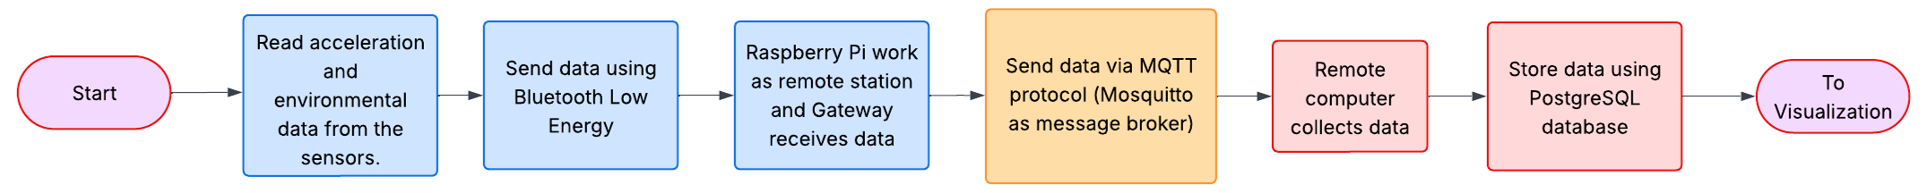
\includegraphics[width=\linewidth]{Methodological_Approach_1_1}
        \caption{}
    \end{subfigure}
    \hfill
    \begin{subfigure}[t]{1.05\textwidth}
        \centering
        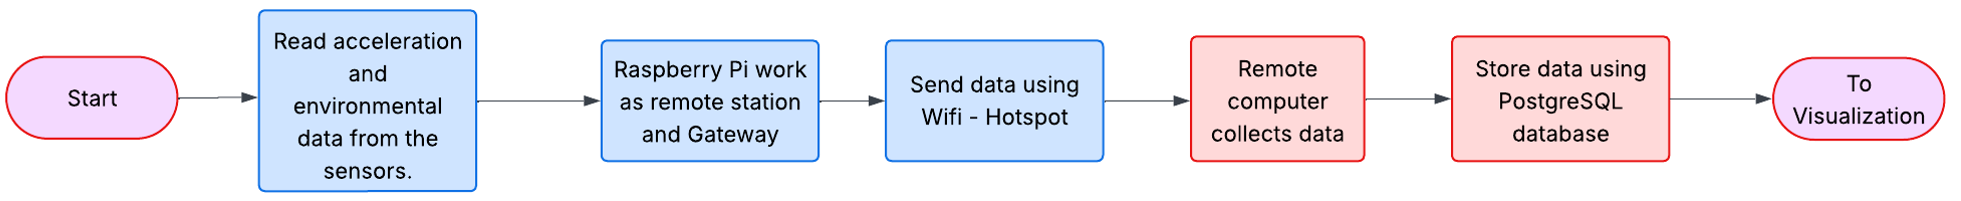
\includegraphics[width=1\linewidth]{Methodological_Approach_2_1}
        \caption{}
    \end{subfigure}
    %\begin{subfigure}[t]{0.30\textwidth}
        %\centering
        %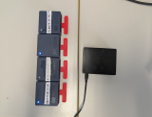
\includegraphics[width=\linewidth]{Methodological_Approach_1_4}
        %\caption{Nordic Thingy:53 sensor node used for data acquisition in the Digital Twin framework.}
    %\end{subfigure}
    \caption{Methodological approach for the digital twin framework: (a) MQTT and PostgreSQL; 
    (b) local data acquisition and processing workflow for wind load assessment of GDR-era heritage buildings.}
    \label{fig:method1}
  \end{center}
\end{figure}

\subsection{Digital Twin framework}

\noindent The conceptual foundation of this work is the Digital Twin paradigm, illustrated
in Figure~\ref{fig:digital_twin}. A Digital Twin is a virtual replica of a
physical system that enables real-time monitoring, analysis, and
decision-making through a closed feedback loop connecting four main components.


The \textbf{Physical Twin} encompasses the real-world assets under study 
objects (buildings and infrastructure), processes (operational workflows), and
systems (interconnected structural components). \textbf{Data collection} forms
the bridge between the physical and digital worlds: sensors, IoT devices, and
measurement instruments continuously capture data from the physical twin and
feed it into the digital entity. The \textbf{Digital Entity} (Virtual Twin) is
the computational replica, built on representative models (3D geometry, BIM,
simulation models), a data management layer for storage and organisation of
incoming records, and data analytics modules for processing and interpretation
(statistical methods, machine learning). Finally, the \textbf{Services,
Information and Decision} stage translates insights from the digital entity
into actionable outputs that are fed back to influence the physical twin,
closing the loop. At the centre of the cycle sits the principle of
human-centric design, emphasising that all stages ultimately serve human
decision-makers.

\begin{figure}[H]
  \begin{center}
    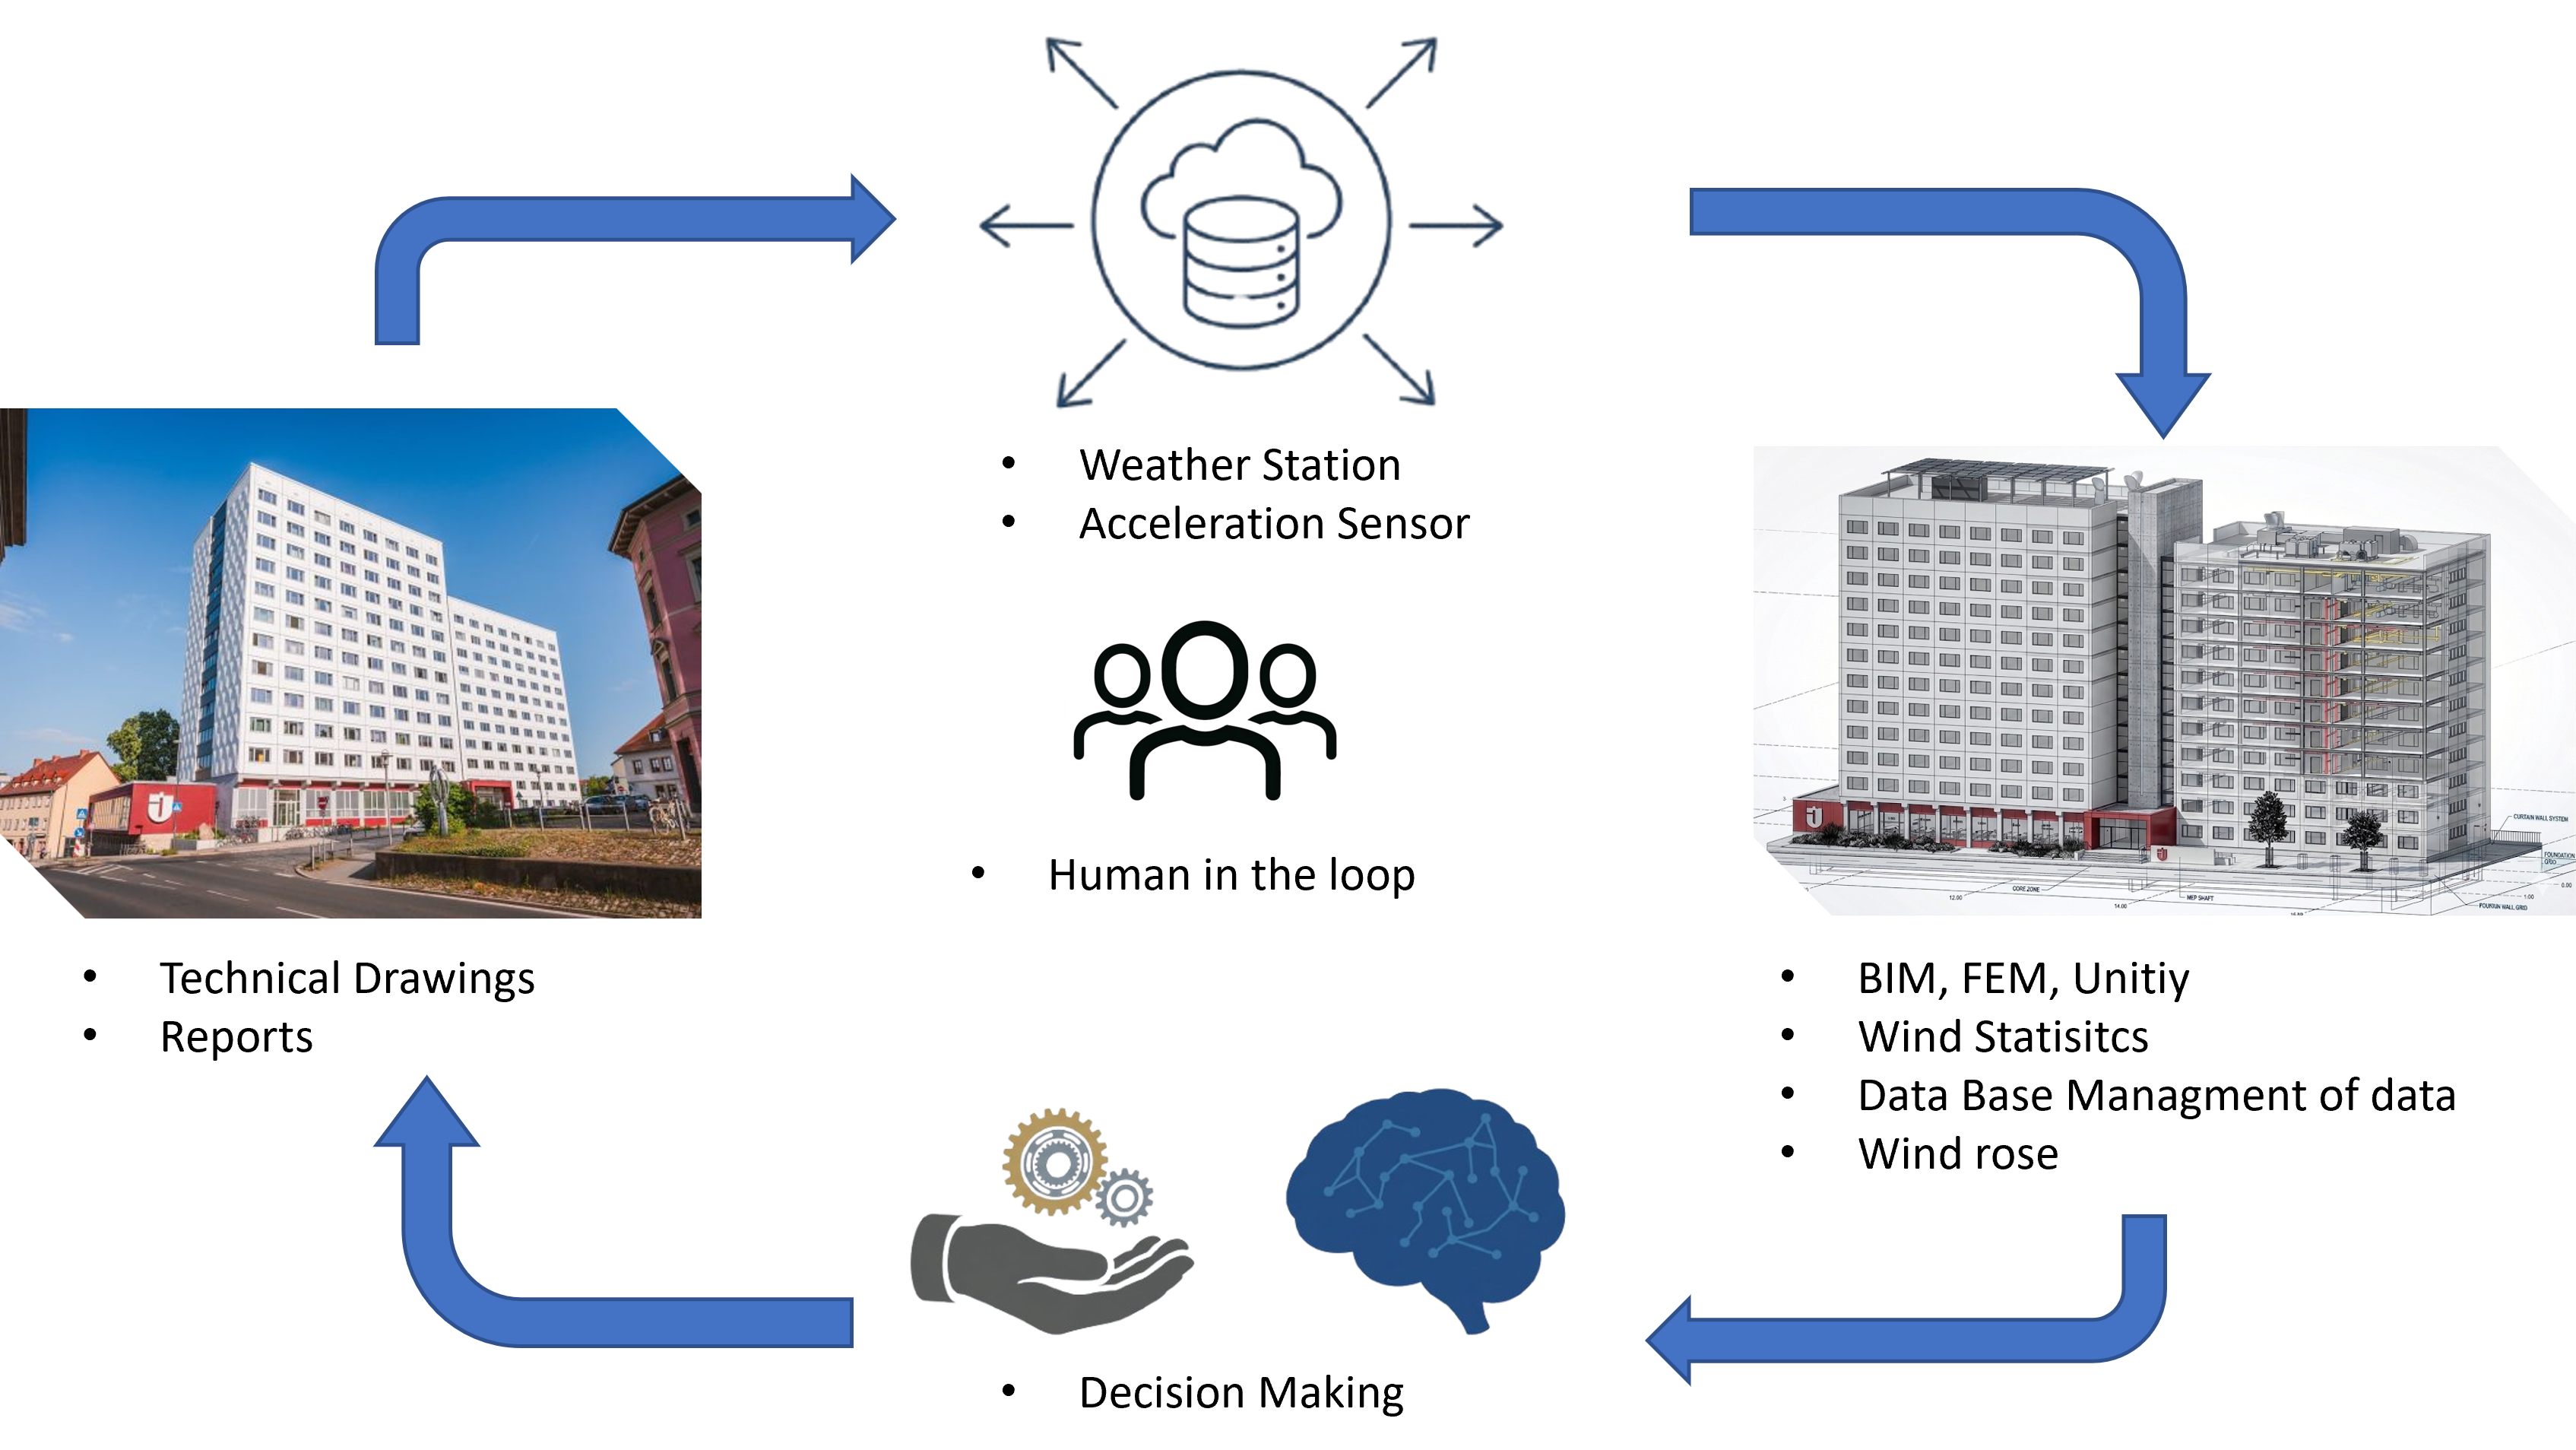
\includegraphics[width=0.85\linewidth]{Digital_Twin}
    \caption{Digital Twin framework}
    \label{fig:digital_twin}
  \end{center}
\end{figure}

%\begin{figure}[H]
%  \begin{center}
%    \begin{subfigure}[t]{0.9\textwidth}
%        \centering
%        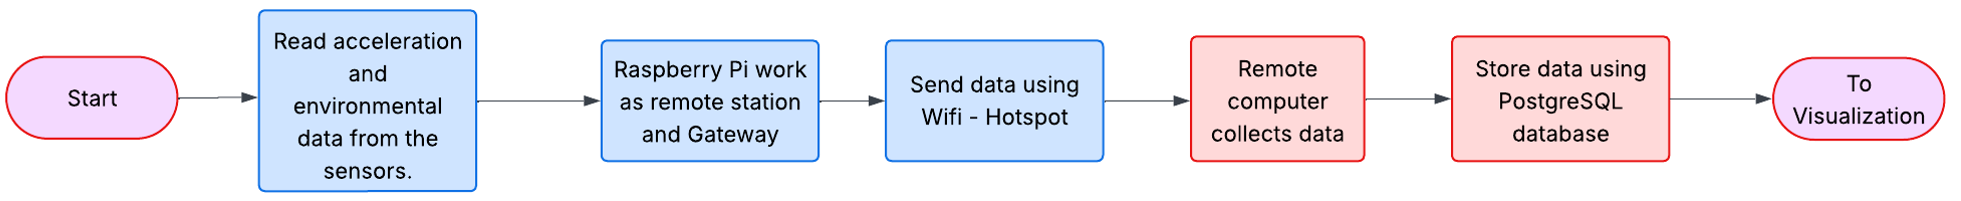
\includegraphics[width=1.1\linewidth]{Methodological_Approach_2_1}
%        \caption{Overall conceptual framework: from physical asset to Digital Twin methodology approach 2.}
%    \end{subfigure}
%    \hfill
%    \begin{subfigure}[t]{0.48\textwidth}
%        \centering
%        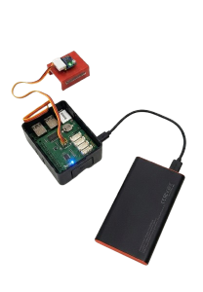
\includegraphics[width=0.55\linewidth]{Methodological_Approach_2_3}
%        \caption{Assembly and deployment of the sensor MPU-6050 and Raspberry Pi.}
%    \end{subfigure}
%    \caption{Methodological Approach 2 --- Sensor hardware development and
%             deployment workflow.}
%    \label{fig:method2}
%  \end{center}
%\end{figure}


\subsection{Signal processing and FFT analysis}

\noindent The recorded acceleration signals were transformed into the
frequency domain using the Fast Fourier Transform (FFT), as given by
Equation~\ref{eq:fft},

\begin{equation}
    X(f_k) = \sum_{n=0}^{N-1} x(n)\, e^{-j\,2\pi k n / N}, \quad
    k = 0, 1, \ldots, N-1
    \label{eq:fft}
\end{equation}

\noindent where $x(n)$ is the $n$-th discrete acceleration sample, $N$ is the total
number of samples, and $f_k = k\,f_s / N$ is the frequency corresponding to
bin $k$ at sampling frequency $f_s$. The dominant peaks in the resulting
spectrum were identified as the principal natural frequencies (modes) of the
structure.




\section{Case Study}
\label{sec:results}

\subsection{Physical Twin of the Jakobsplan building}

[To be completed by Singh.]


\begin{figure}[H]
  \begin{center}
    \begin{subfigure}[t]{0.48\textwidth}
        \centering
        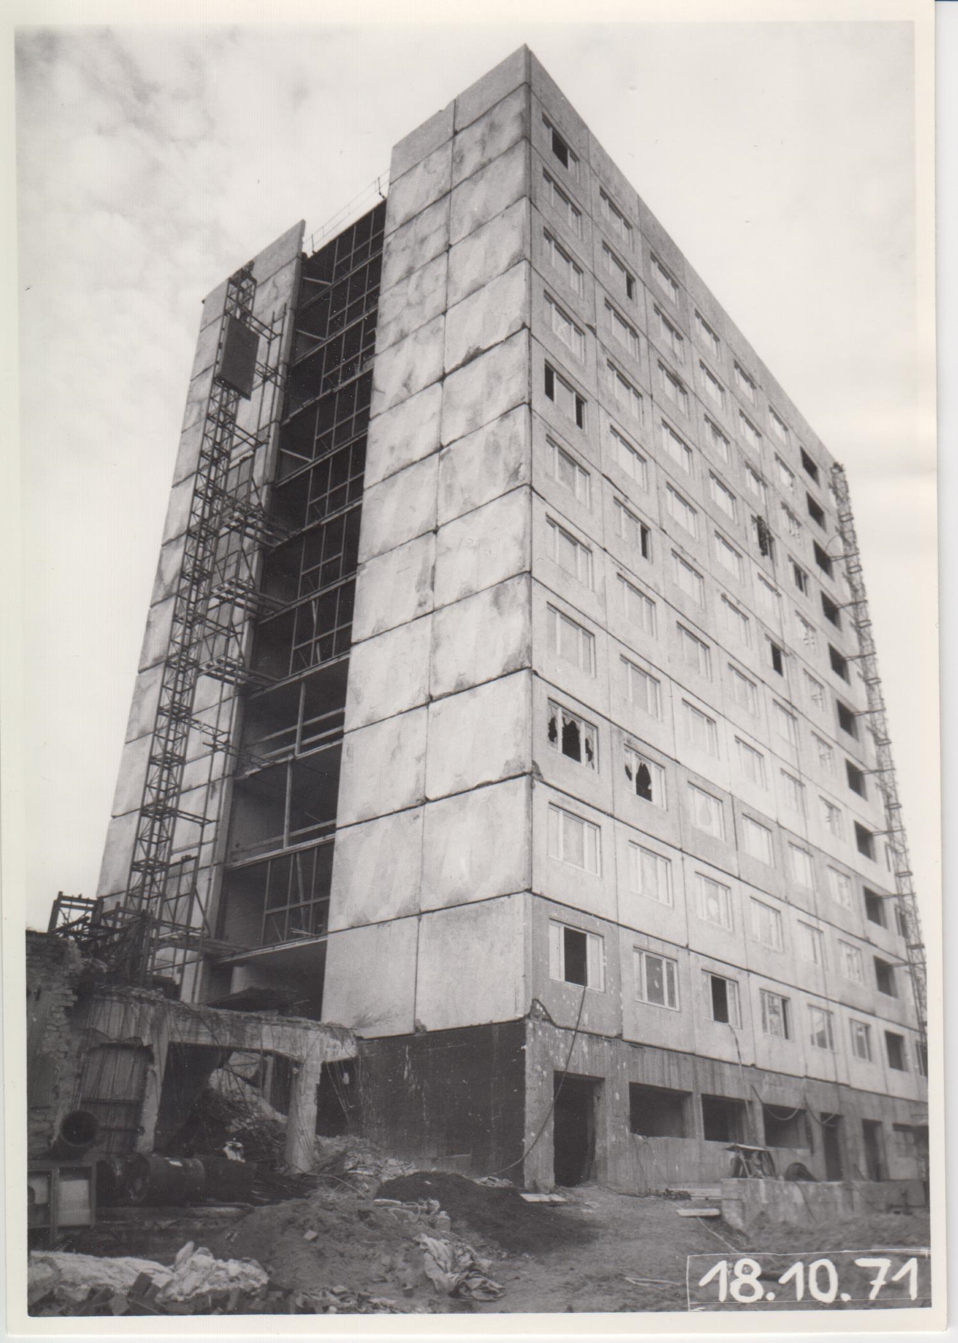
\includegraphics[width=0.65\linewidth]{Implementation_Jakobsplant_Photos_5}
        \caption{Exterior view of the Jakobsplan complex during construction (1971).}
    \end{subfigure}
    \hfill
    \begin{subfigure}[t]{0.48\textwidth}
        \centering
        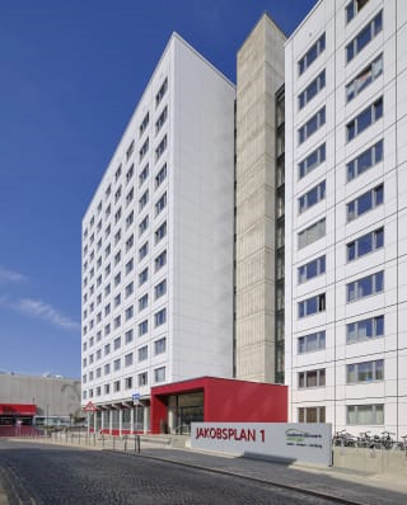
\includegraphics[width=0.75\linewidth]{Implementation_Jakobsplant_Photos_1}
        \caption{Exterior view of the Jakobsplan complex after renovation (current state).}
    \end{subfigure}
    \caption{Jakobsplan building, Weimar --- photographic documentation of the
             case-study structure.}
    \label{fig:jakobsplant_building}
  \end{center}
\end{figure}

\subsection{Data Collection}

[To be completed by Cesar and Itzel.] \\


\noindent\textbf{Weather Station}

\noindent [To be completed by Itzel.] \\


\subsubsection{Sensor node design and assembly}

\noindent Three hardware platforms were evaluated for low-cost ambient-vibration data
acquisition, each paired with a suitable acceleration sensor. The primary
platform is the \textbf{Nordic Thingy:53}, a dedicated IoT prototyping module
based on the Nordic nRF5340 dual-core SoC, which integrates an \textbf{ADXL362}
ultra-low-power three-axis MEMS accelerometer (Analog Devices) providing
tri-axial linear acceleration; data are transmitted wirelessly via Bluetooth
Low Energy~5.2. The second platform, used in Methodological Approach~2,
consists of a \textbf{Raspberry Pi Zero W} a single-core 1\,GHz
single-board computer with 512\,MB RAM and 802.11n Wi-Fi running a full
Linux environment connected to an external \textbf{MPU-6050} six-axis
MEMS IMU via I\textsuperscript{2}C at up to 1\,kHz sampling rate. In this configuration 
the Raspberry Pi Zero W acts as both the sensor controller and the local data logger, transmitting the collected 
records over the local network. In Methodological Approach~1, a \textbf{Raspberry Pi 3B} serves as
the central gateway, managing either Thingy:53 or MPU-6050 nodes; its
quad-core 1.2\,GHz processor and 1\,GB RAM provide the processing capacity
required for real-time data routing and storage, and data are forwarded using
the MQTT protocol with Mosquitto as the message broker. As an additional
low-cost alternative, an \textbf{ESP32} dual-core 240\,MHz microcontroller
with integrated Wi-Fi and Bluetooth was coupled with the MPU-6050 via
I\textsuperscript{2}C to broaden the comparison of sensor-platform
combinations. For the purposes of this study, only the accelerometer channels
$a_x$, $a_y$, and $a_z$ were used across all platforms, with a full-scale
range set to $\pm$\,2\,$g$. The assembled devices are illustrated in Figure~\ref{fig:assembly}.


\begin{figure}[ht]
  \begin{center}
    \begin{subfigure}[t]{0.3\textwidth}
        \centering
        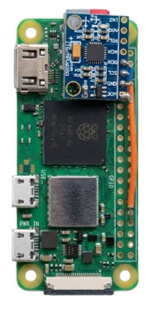
\includegraphics[width=0.85\linewidth]{Implementation_1}
        \caption{Raspberry Pi Zero W and MPU-6050 module.}
    \end{subfigure}\hfill
    \begin{subfigure}[t]{0.3\textwidth}
        \centering
        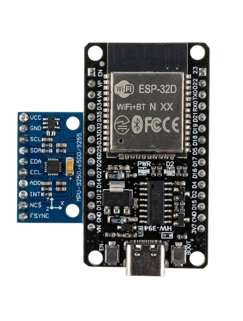
\includegraphics[width=\linewidth]{Implementation_2}
        \caption{Soldering the MPU-6050 to ESP32.}
    \end{subfigure}\hfill
    \begin{subfigure}[t]{0.3\textwidth}
        \centering
        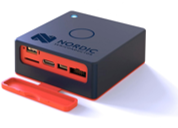
\includegraphics[width=\linewidth]{Implementation_3}
        \caption{Thingy-53 sensor unit.}
    \end{subfigure}\\[6pt]
    %\begin{subfigure}[t]{0.3\textwidth}
    %    \centering
    %    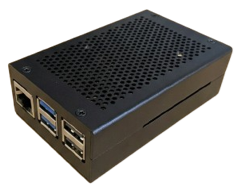
\includegraphics[width=\linewidth]{Implementation_4}
    %    \caption{Raspberry Pi 3B gateway.}
    %\end{subfigure}\hfill
    %\begin{subfigure}[t]{0.3\textwidth}
    %    \centering
    %    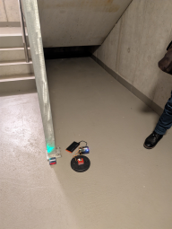
\includegraphics[width=0.85\linewidth]{Implementation_6}
    %    \caption{3D-printed enclosure design.}
    %\end{subfigure}\hfill
    %\begin{subfigure}[t]{0.3\textwidth}
    %    \centering
    %    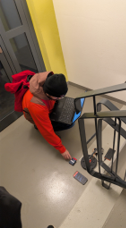
\includegraphics[width=0.6\linewidth]{Implementation_7}
    %    \caption{Board inserted into enclosure.}
    %\end{subfigure}
    \caption{Assembly of the low-cost IoT sensor:
             Raspberry Pi, ESP32 microcontroller with MPU-6050 tri-axial accelerometer and Thingy - 53.}
    \label{fig:assembly}
  \end{center}
\end{figure}




\subsubsection{Firmware and data acquisition}

\noindent The firmware for the Thingy:53 nodes was written in C using the nRF Connect SDK
and manages the following tasks: (1) accelerometer initialisation and configuration;
(2) timestamped sample acquisition at 400\,Hz; (3) local buffering in SRAM; and
(4) periodic data transmission to the Raspberry Pi 3B gateway via Bluetooth Low
Energy~5.2. A companion Python application running on the Raspberry Pi 3B handled
device management and forwarded the received data to a Mosquitto MQTT broker.
For the Raspberry Pi Zero W / MPU-6050 nodes, the acquisition and transmission
pipeline was implemented entirely in Python: the script reads accelerometer samples
over I\textsuperscript{2}C at 400\,Hz and publishes them directly to the same MQTT
broker over Wi-Fi. This client--broker architecture decouples data collection from
storage and post-processing, and allows multiple nodes to operate simultaneously
without mutual interference. All raw acceleration records were persisted in a
\textbf{PostgreSQL} relational database, with a schema designed to store
timestamped tri-axial acceleration samples indexed by node identifier and
measurement session.

\subsubsection{Sensor placement in the Jakobsplan building}
\label{sec:placement}

\noindent Sensor positions were selected to try to capture the dominant translational and
torsional modes of the building. The nodes were mounted at representative
floor levels along the height of the structure, with the sensors rigidly fixed
to the concrete slab surfaces to ensure good kinematic coupling and to minimise
measurement artefacts from local resonances of the mounting system. The exact
positions and the corresponding coordinate system are detailed in
Figure~\ref{fig:sensor_positions}.

\begin{figure}[H]
  \begin{center}
    \begin{subfigure}[t]{\textwidth}
        \centering
        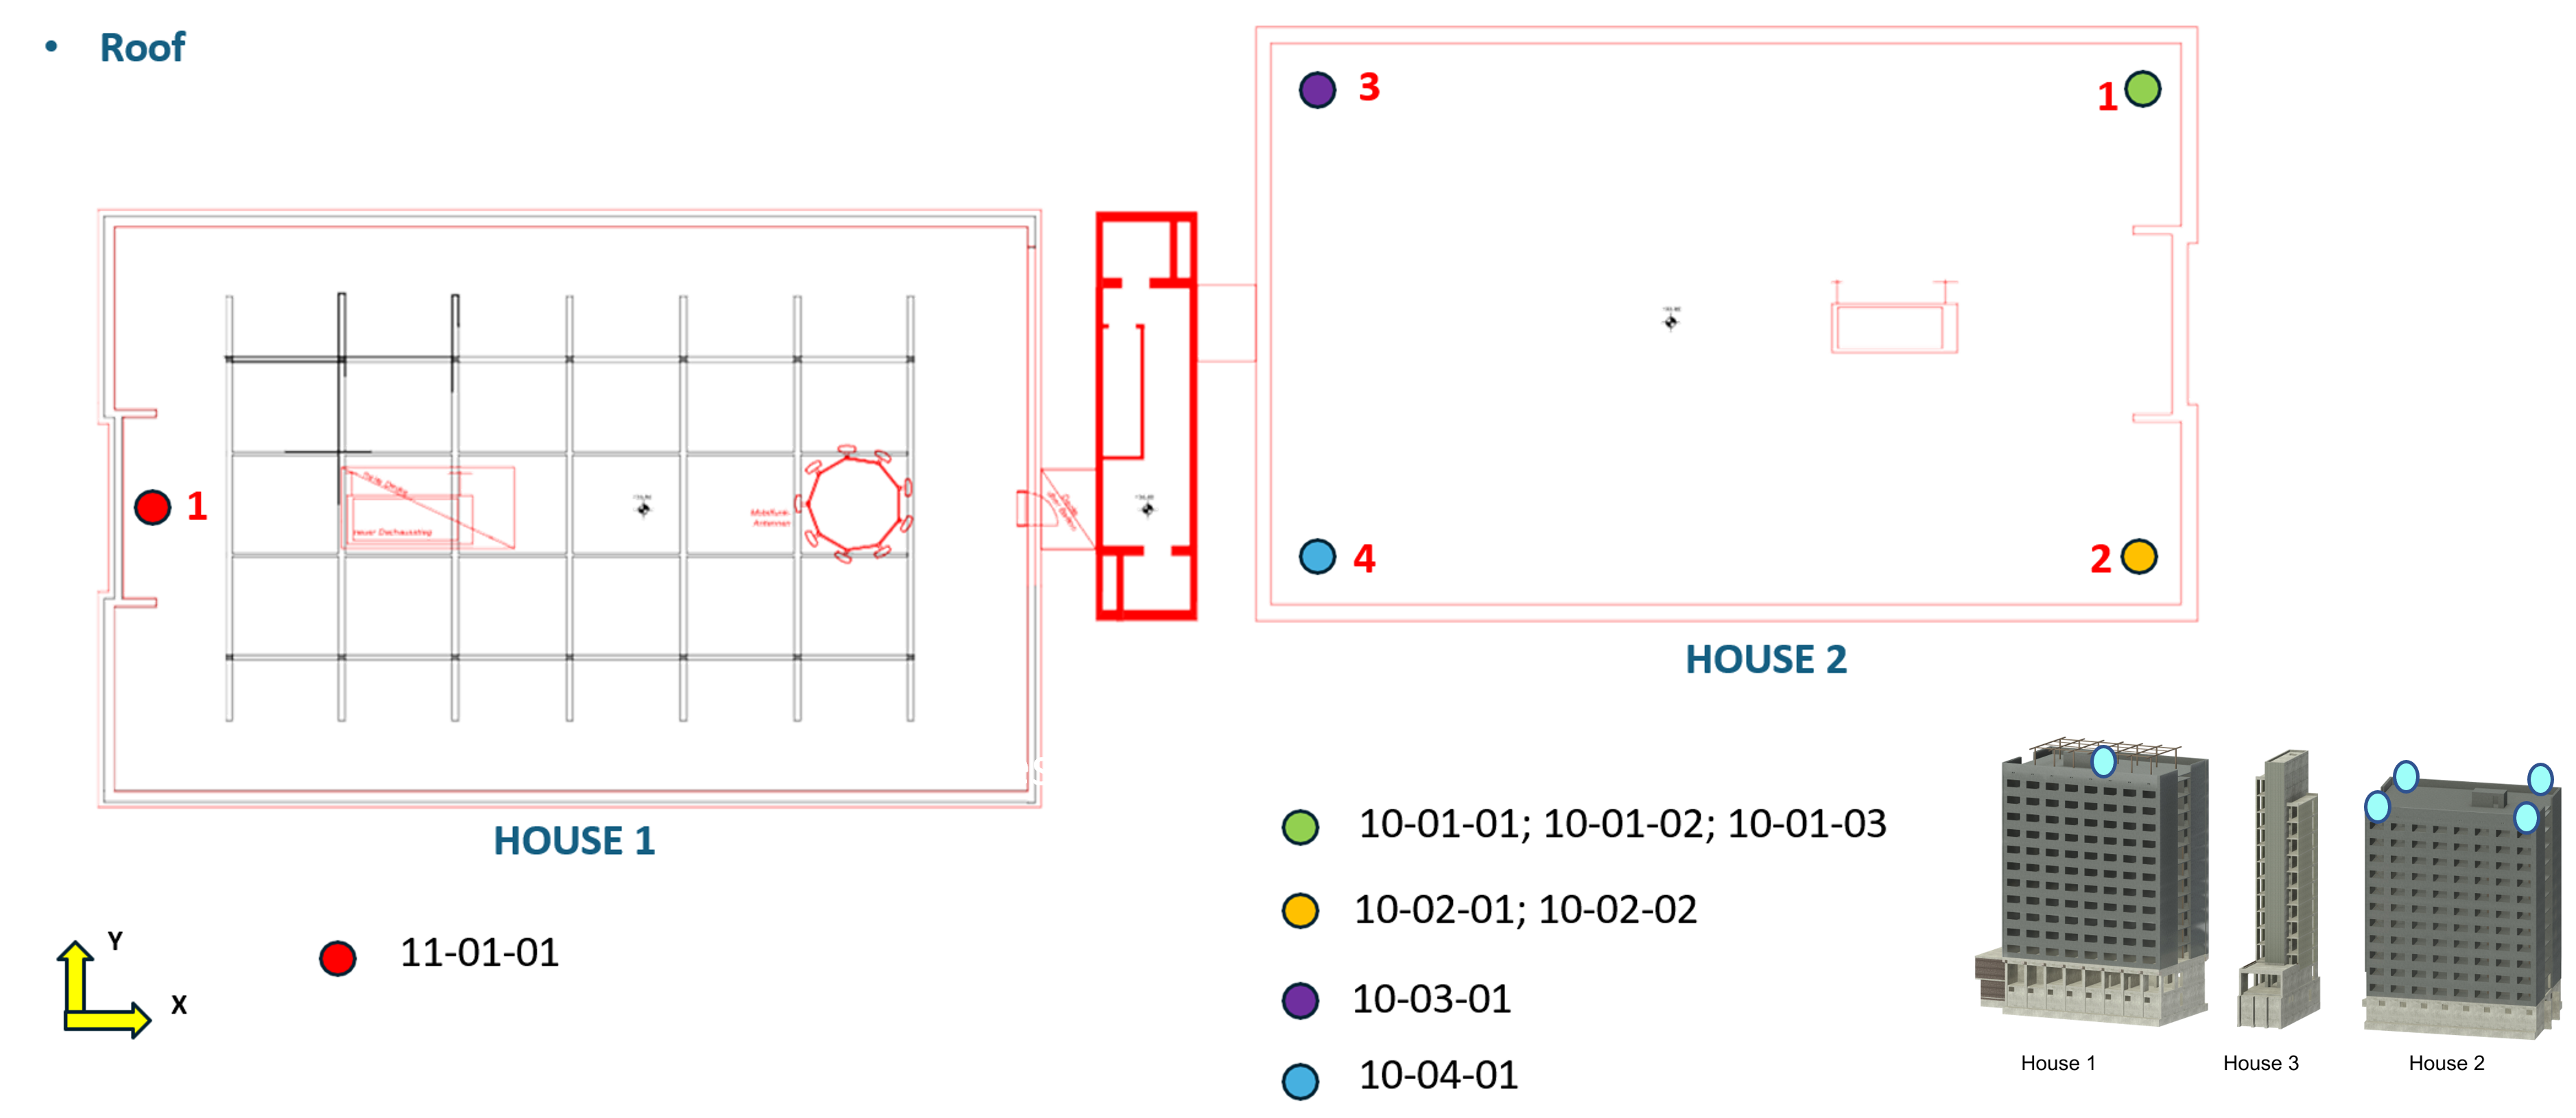
\includegraphics[width=0.7\linewidth]{position_sensors_DataPostproccesing_1}
        \caption{Floor plan showing sensor locations.}
    \end{subfigure}\\[6pt]
    \begin{subfigure}[t]{\textwidth}
        \centering
        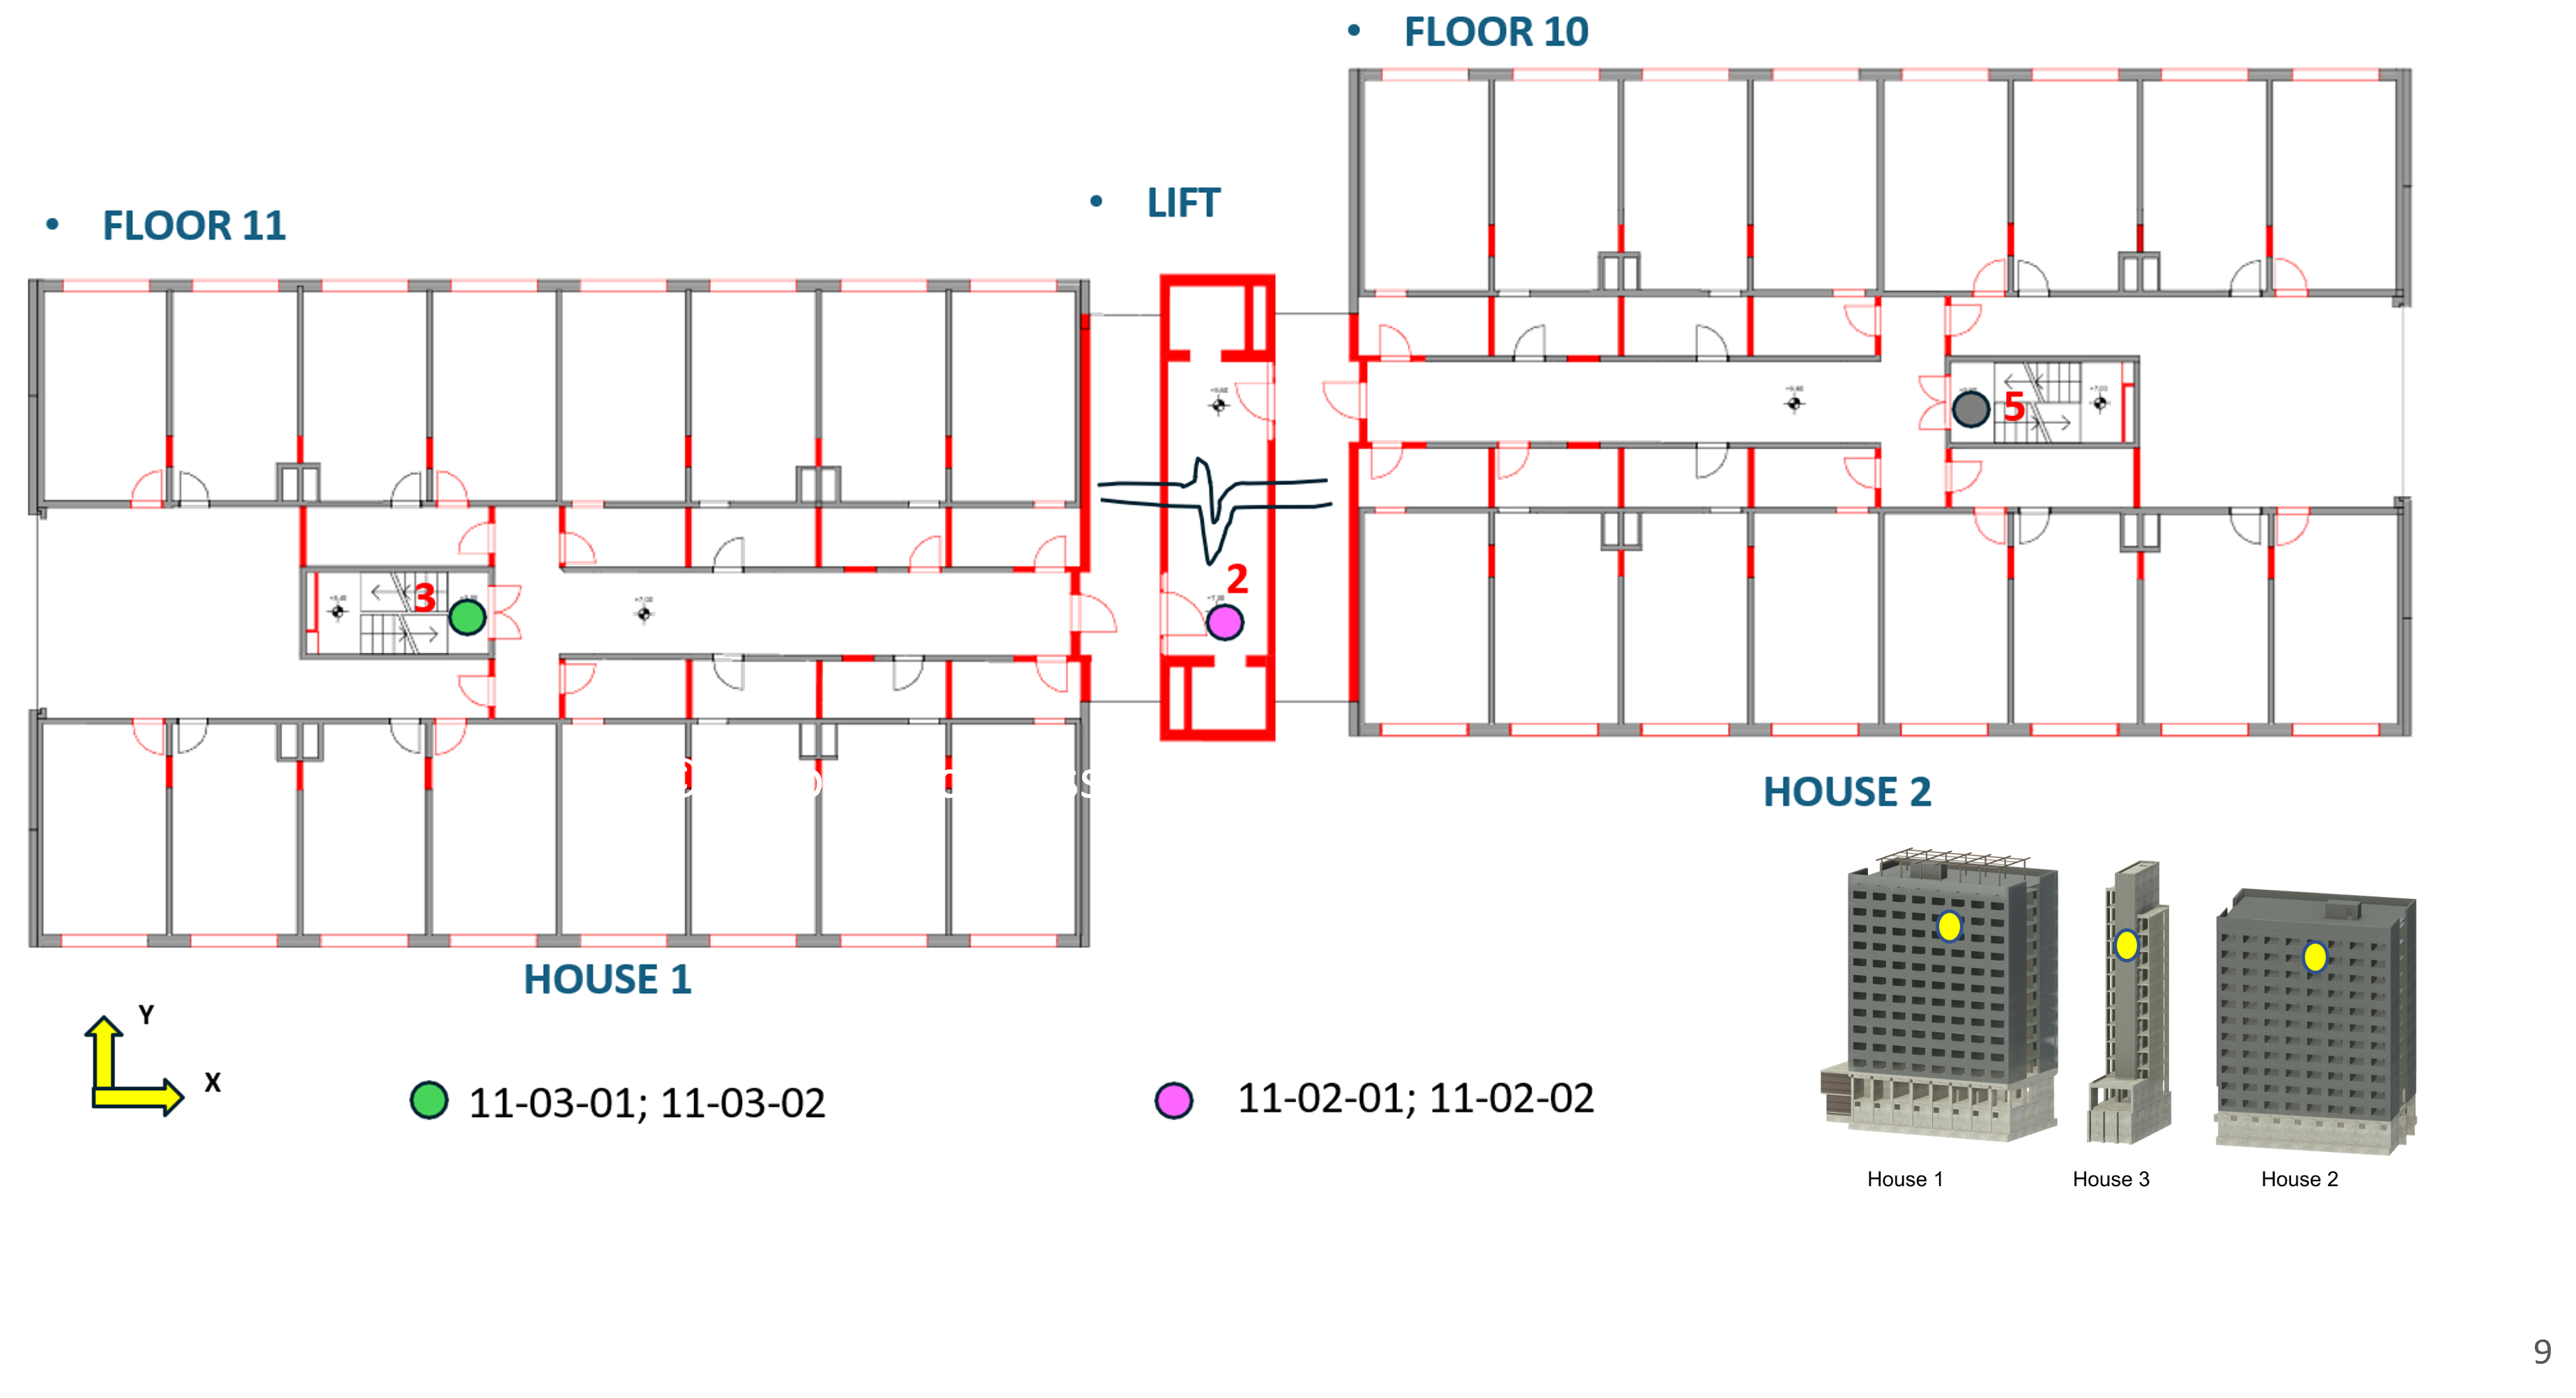
\includegraphics[width=0.7\linewidth]{position_sensors_DataPostproccesing_2}
        \caption{Elevation view of sensor mounting heights.}
    \end{subfigure}\\[6pt]
    \begin{subfigure}[t]{\textwidth}
        \centering
        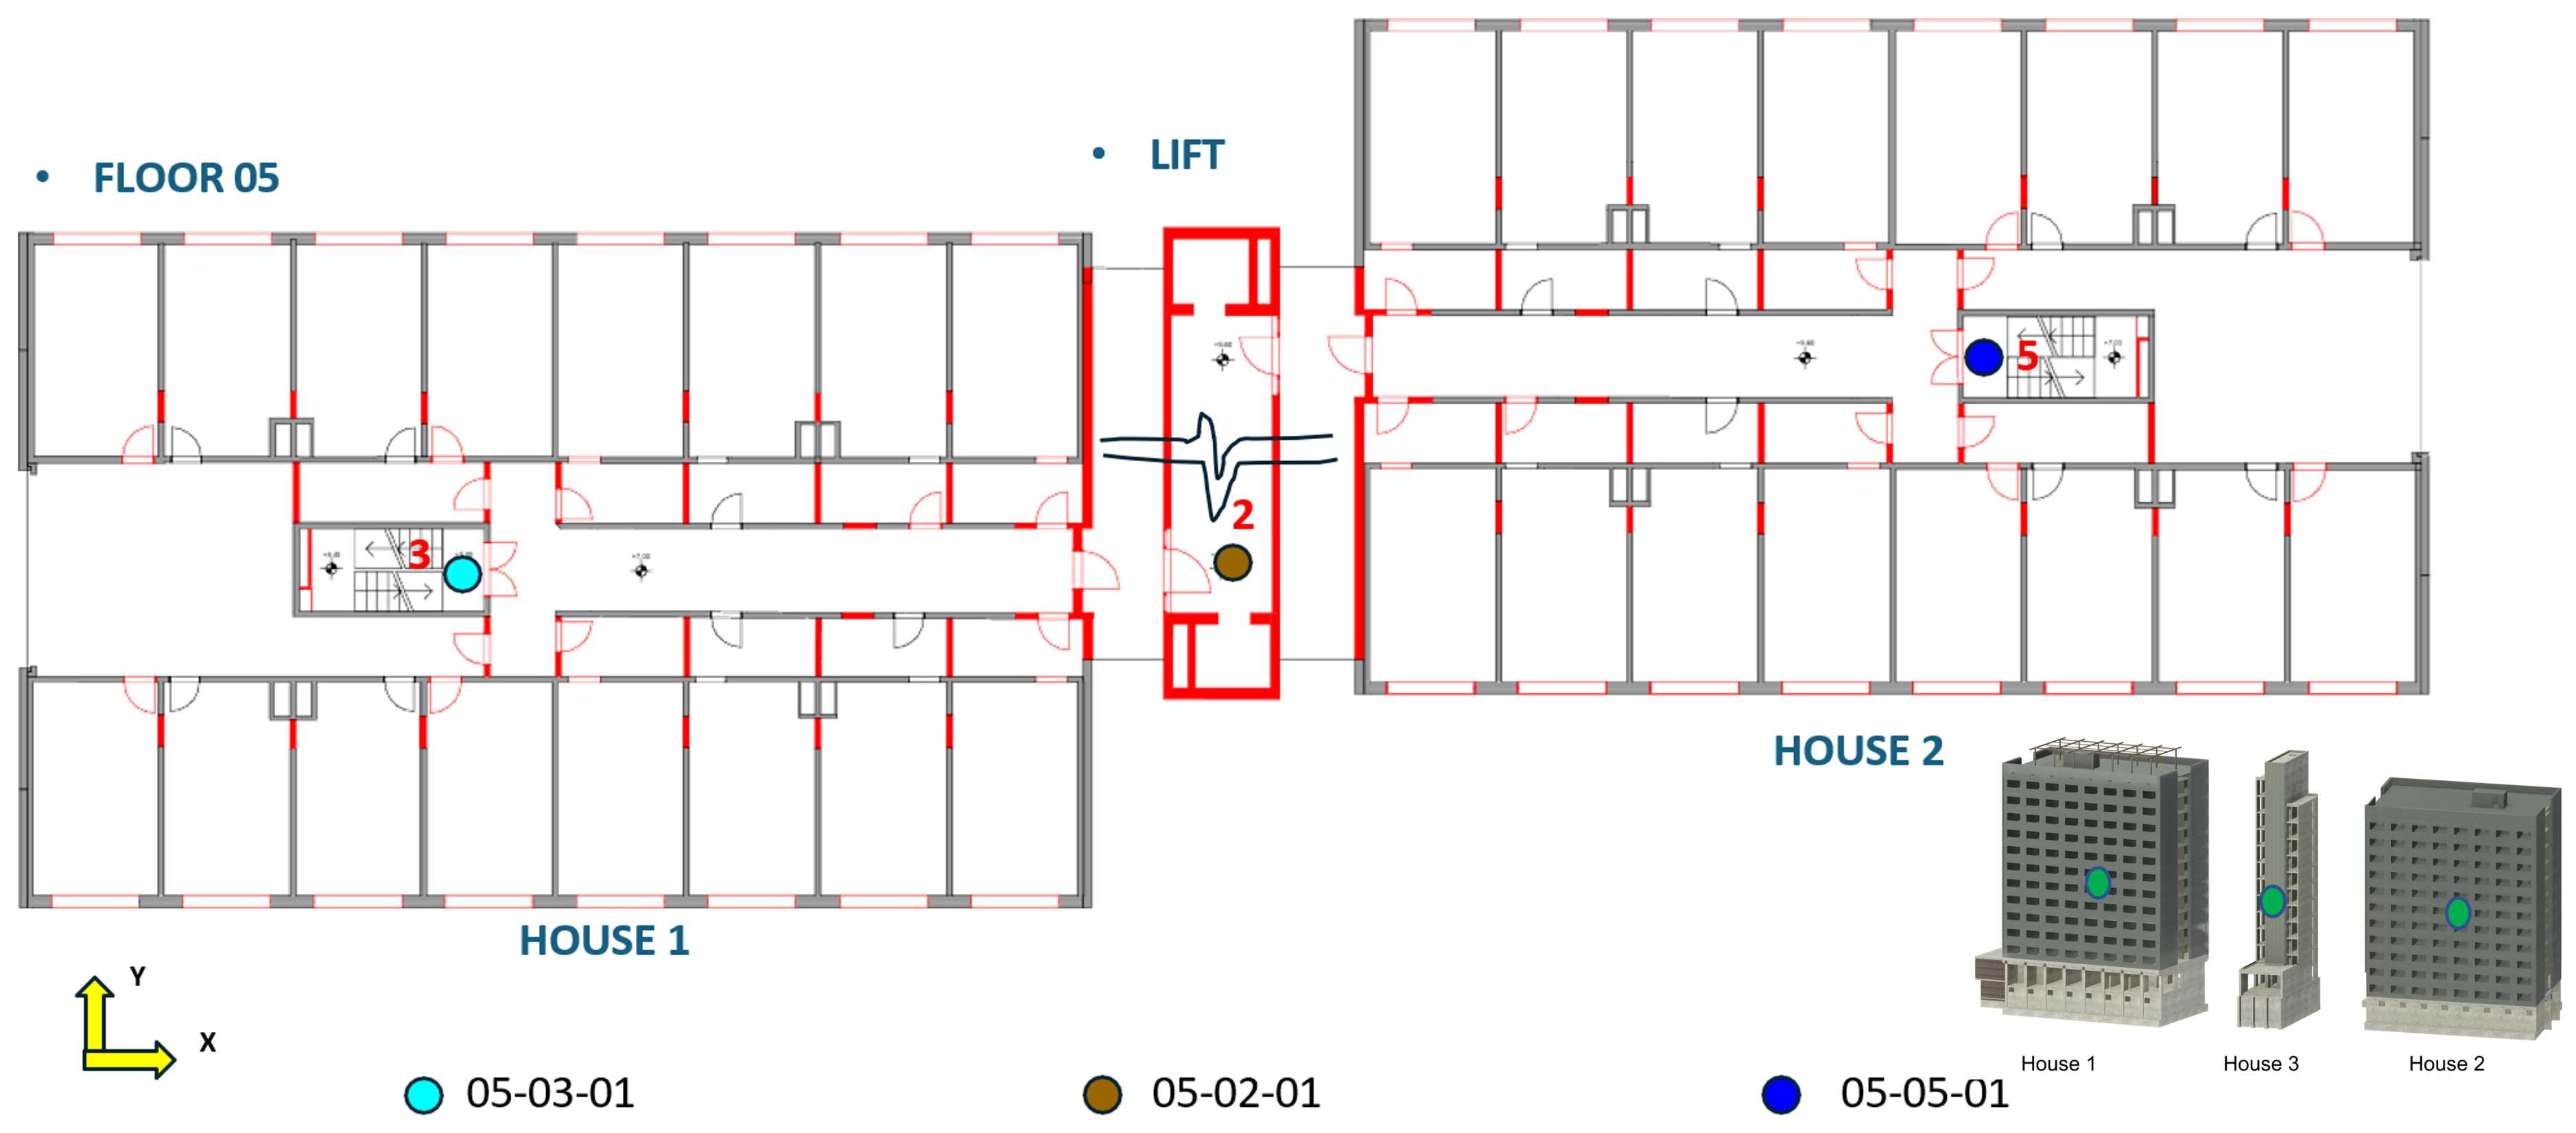
\includegraphics[width=0.7\linewidth]{position_sensors_DataPostproccesing_3}
        \caption{Data post-processing pipeline.}
    \end{subfigure}
    \caption{Sensor positions within the Jakobsplan building and
             corresponding data post-processing workflow.}
    \label{fig:sensor_positions}
  \end{center}
\end{figure}

\subsection{Virtual Twin}

\noindent [To be completed Singh BIM and FEM model.]
\subsubsection{Wind statistics}
\noindent [To be completed by Itzel.]
\subsubsection{BIM and FEM model}
\noindent [To be completed by Singh.]
\subsubsection{Data Base management and visualization}
\noindent [To be completed by Cesar.]

\subsubsection{Data Processing}
\noindent [To be completed by Itzel.]

put fft and PSD
\subsection{Human Loop and decision making}

\noindent [To be completed by Anastasia.]





\begin{table}[ht]
  \begin{center}
    \begin{tabular}{@{}clcc@{}}
      \toprule
      Mode & Description & Direction & $f_n$ (Hz) \\
      \midrule
      1 & First translational (longitudinal) & $x$ & --- \\
      2 & First translational (transverse)   & $y$ & --- \\
      \bottomrule
    \end{tabular}
  \end{center}
  \caption{Natural frequencies identified from ambient vibration measurements
           at the Jakobsplan building. Values to be completed following final
           post-processing.}
  \label{tab:frequencies}
\end{table}

\section{Conclusions and future work}
\noindent [To be completed.]

\section*{Acknowledgements} 
\noindent [To be completed.]

\printbibliography{}

\end{document}
